\chapter{Introducción}

En este artículo presentamos una herramienta capaz de automatizar el diseño del señalamiento y la implementación del sistema de enclavamiento ferroviario para cualquier locación, dado únicamente el diseño de su traza ferroviaria. Se discutiran los detalles del diseño de la herramienta, su arquitectura, casos de uso y aplicaciones en locaciones teóricas y reales.

\section{Sistemas ferroviarios}

    Las redes ferroviarias modernas presentan dos elementos fundamentales en su infraestructura: una topología y elementos ferroviarios. La topología es el entramado de vías férreas conectadas de forma arbitraria, cuyo diseño busca cumplir una función particular, interconectando diversos elementos ferroviarios. Estos elementos pueden ser para determinar la ubicación del tren, para delimitar la circulación de vehículos en cruces ferroviarios, permitir el ascenso y descenso de pasajeros, o para modificar dinámicamente los caminos por los que los trenes circulan, entre otras funciones.

    Cualquiera sea el elemento involucrado, altera las funciones de la red y su inminente proximidad debe informarse cuanto antes al conductor del tren. Este podrá decidir, de estar permitido, modificar o no su accionar antes de alcanzar dicho elemento. Es tarea del señalamiento ferroviario alertar a los conductores ferroviarios de cualquier elemento que pueda representar un peligro, evitando así colisiones con otras formaciones o descarrilamientos en zonas críticas. El señalamiento ferroviario incluye un elemento fundamental: los semáforos.

    Los semáforos (de ahora en mas denominados "señales"), constituyen el medio de comunicación primario entre los conductores y su entorno, informándoles de la habilitación o denegación de uso de las vías posteriores mediante su color, denominado aspecto. Cada señal puede presentar un único aspecto por vez de un conjunto posible que varía según el país o la región. Los aspectos utilizados en Argentina son el verde (permitido avanzar), amarillo (atención) y rojo (detenerse). Algunas señales pueden no tener el aspecto verde (señales de maniobras de dos aspectos) o incorporar un aspecto extra entre el rojo y el amarillo (señales de cuatro aspectos que incluyen el doble amarillo).
    
    Dos señales consecutivas con la misma dirección y sentido constituyen una ruta ferroviaria. Los operarios ferroviarios solicitan al sistema de enclavamientos las rutas que necesitan en base a la logística deseada. El sistema de enclavamientos habilitará o denegará las rutas solicitadas en función del estado de los elementos ferroviarios cercanos y de las demás rutas activas. Esta función es vital para el sistema ferroviario y su fin último es permitir la circulación de trenes de la forma mas segura o, de no ser posible, no permitir circulación alguna.

    El diseño de los sistemas de señalamiento es un proceso complejo que involucra, principalmente, tres etapas: el análisis de la red ferroviaria, la detección de zonas de mayor probabilidad de descarrilamientos y colisiones, y la óptima localización de las señales correctas para cada función [REF]. La generación automática del señalamiento es de gran importancia y utilidad para el desarrollo de redes ferroviarias nuevas o para revitalizar redes ferroviarias abandonadas o en desuso. Es relevante incluso en redes ferroviarias que son alteradas debido a la adición, modificación o eliminación de elementos ferroviarios tales como pasos a nivel o plataformas, lo cual implica que el señalamiento debo actualizarse en consecuencia.

\subsection{Principios de señalamiento ferroviario}
    
    El proceso de diseño del señalamiento requiere reglas claras y bien definidas sobre cuántas señales colocar, dónde colocar cada señal, bajo que condiciones, de qué tipo deben ser las señales, cómo deben orientarse, etc. Lamentablemente, el criterio utilizado a la hora de definir el señalamiento dista de ser uniforme de nación a nación. La obligatoriedad de ciertas señales, la protección de ciertos elementos, el granularidad de la red o incluso el tener las reglas por escrito son factores que cambian al atravesar las fronteras de cada país. Esto implica, claramente, una barrera enorme al tratar de integrar las redes ferroviarias transnacionales, como en el caso Europeo durante formación de la Unión Europea[REF].
    
    Para la realización de este trabajo se optó por recurrir al Instituto de Ingenieros en Señalamiento Ferroviario (IRSE, por sus siglas en inglés) [IRSE] y a la Junta de Normas y Seguridad de la Industria Ferroviaria (RISSB, por sus siglas en inglés) [RISSB]. Los reglamentos de diseño y definiciones de estas organizaciones son aceptadas por una gran cantidad de empresas del sector ferroviario y autoridades de gran peso. Entre ellas, por la agencia de transporte de Nueva Gales del Sur, en Australia (TfNSW, por sus siglás en inglés) [TfNSW]. De ésta última se recopilaron los siguientes principios de diseño ferroviario:
    
    \begin{itemize}
        \item [($P_1$)] Principio de autoridad: el derecho del tren a circular esta limitada a una pequeña porción de la infraestructura.
        \item [($P_2$)] Principio de claridad: las autoridades otorgadas o negadas no deben ser ambiguas. 
        \item [($P_3$)] Principio de anticipación: los conductores de trenes deben ser advertidos de los peligros cercanos con el suficiente tiempo para reaccionar.
        \item [($P_4$)] Principio de granularidad: las rutas deben ser lo mas cortas posibles.
        \item [($P_5$)] Principio de terminalidad: los conductores de trenes deben ser advertidos cuando se encuentren circulando próximos al final de la red.
        \item [($P_6$)] Principio de infraestructura: los conductores de trenes deben ser advertidos de cualquier infraestructura dinámica o estática próxima.
        \item [($P_7$)] Principio de no bloqueo: se debe evitar en todo momento que los trenes bloqueen el acceso a la infraestructura o ramificaciones a otros tresnes, de ser posible.
    \end{itemize}

    La totalidad del análisis realizado en este proyecto se basa en los principios expuestos. Se puede deducir de los mismos que un sistema de señalamiento debe proteger cada elemento ferroviario ($P_1$,$P_5$,$P_6$), en cada dirección posible ($P_3$,$P_7$). Por lo tanto debemos considerar la posibilidad de que cada tramo de vía puede ser transitado en ambos sentidos. Esto implica a su vez considerar todas las rutas posibles soportadas por la red ferroviaria, y no solamente las necesarias desde un punto de vista logístico.
\subsection{Elementos ferroviarios}

El sistema ferroviario consta de diversos elementos que incluyen la infraestructura (tendido ferroviario, plataformas, cruces de vía), sensores (circuitos de vía, contadores de eje), actuadores (barreras ferroviarias, máquinas de cambios) e interfaces visuales con los conductores (semáforos ferroviarios). Todos estos elementos se interrelacionan y funcionan en conjunto dentro del sistema de señalamiento y el sistema de enclavamiento. Cada uno de estos elementos será descripto en la sucesivas secciones, en orden tal de integrar los conceptos anteriores de la forma mas clara posible.

\subsubsection{Vías}

Las vías férreas son el elemento ferroviario mas esencial, son la columna vertebral de la infraestructura ferroviaria. Estas constituyen el sitio por el cual se desplazan los trenes, definiendo no solo la dirección del desplazamiento, sino también restringiendo el dominio del tren. Esto lo diferencia de otros medios de transporte como el automóvil que no necesitan un camino para circular y, aún teniendo una carretera, puede moverse libremente por fuera de esta.

Las vías se encuentran separadas por una distancia fija que se mide desde sus caras internas, denominada trocha (Figura \ref{fig:vias_1}). Solamente las formaciones compatibles con ese parámetro de trocha pueden circular por el tendido ferroviario. El valor de la trocha puede variar entre las denominadas trocha angosta (600 a 1372 mm, estándar imperial británico) y trocha ancha (1520 a 3000 mm, estándar ruso, indio, ibérico, irlandés). Se estableció el valor intermedio de 1425 mm como valor de trocha internacional, usado ampliamente en Europa, Norteamérica y Oceanía.

    \begin{figure}[!h]
        \centering
        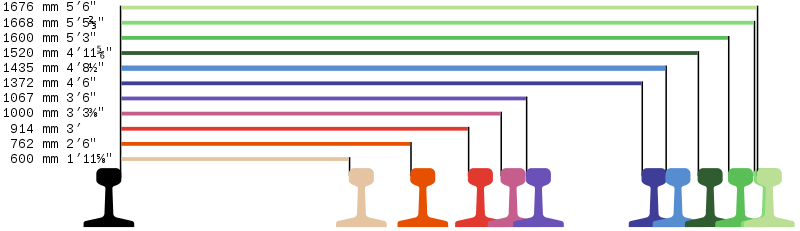
\includegraphics[width=1\textwidth]{Figuras/trocha.png}
        \centering\caption{Vías ferroviarias y trocha.}
        \label{fig:vias_1}
    \end{figure}
    
Existen limitaciones logísticas y físicas por las cuales el tendido ferroviario no puede ser un continuo rígido. En primer lugar, las vías deben ser de un tamaño acotado, tal que puedan transportarse a la locación donde serán instaladas en tramos rectos o curvos. En segundo lugar, la dilatación y contracción de las vías debido a los cambios de temperatura añaden una restricción respecto a la distancia mínima que deben tener entre las mismas. De lo contrario, la dilatación del material puede provocar daños irreparables a la infraestructura y estos, a su vez, ser motivo de descarrilamientos, como ya ha ocurrido en los comienzos de la industria ferroviaria [REF]. 
    
Cada vía puede ser clasificada en dos grupos: vías ascendentes o vías descendentes (\ref{fig:vias_2}). Las ascendentes son aquellas por las cuales los trenes circulan únicamente en la dirección del kilometraje en sentido creciente. Las descendentes son aquellas por las cuales los trenes circulan únicamente en la dirección del kilometraje en sentido decreciente [REF]. 

    \begin{figure}[!h]
        \centering
        \includegraphics[width=1\textwidth]{example-image}
        \centering\caption{Vías ascendentes y descendentes.}
        \label{fig:vias_2}
    \end{figure}

El kilómetro 0 es la estación principal de la línea ferroviaria, como pueden ser las terminales de Plaza Constitución (para la línea Roca), Once de septiembre (para la línea Sarmiento) y Retiro (para las líneas Mitre y San Martín).  Existen vías de maniobra que pueden ser tanto ascendentes como descendentes. Estas vinculan, mediante un cambio de vías, una sección ascendente con otra descendente, en la cual los trenes deben circular a una velocidad reducida. 

Las vías se agrupan en secciones que, por cuestiones de seguridad y logística, se establece que solo pueden ser utilizadas por un tren a la vez. Estas secciones pueden ser de varios kilómetros en zonas rurales o unos pocos cientos de metros en zonas urbanas, donde la red necesita una mayor granularidad debido a la densidad del tráfico ferroviario en las grandes urbes.
\subsubsection{Fin de vía y transiciones}

\lipsum[1]

\lipsum[1]
\includegraphics{example-image}
\lipsum[1]
\subsubsection{Sistemas de detección de formaciones ferroviarias}

Es de vital importancia que el sistema pueda determinar la posición de un tren dentro del tendido ferroviario. De esta manera, poder habilitar la circulación en secciones donde no exista peligro de colisión con otros formaciones o, por el contrario, detener la marcha de las formaciones anteriores para evitar accidentes. Existen diversas maneras de detectar la posición de un tren, entre ellas el uso de circuitos de vía y contadores de ejes. 

Los circuitos de vía (Figura \ref{fig:deteccion_1}) son dispositivos electrónicos que aplican una diferencia de potencial finita entre los rieles. Cuando una formación ingresa a la sección, sus ruedas metálicas cortocircuitan ambos rieles. El cortocircuito es detectado por el relé y este, a su vez, reporta el estado al resto del sistema. 

    \begin{figure}[!h]
        \centering
        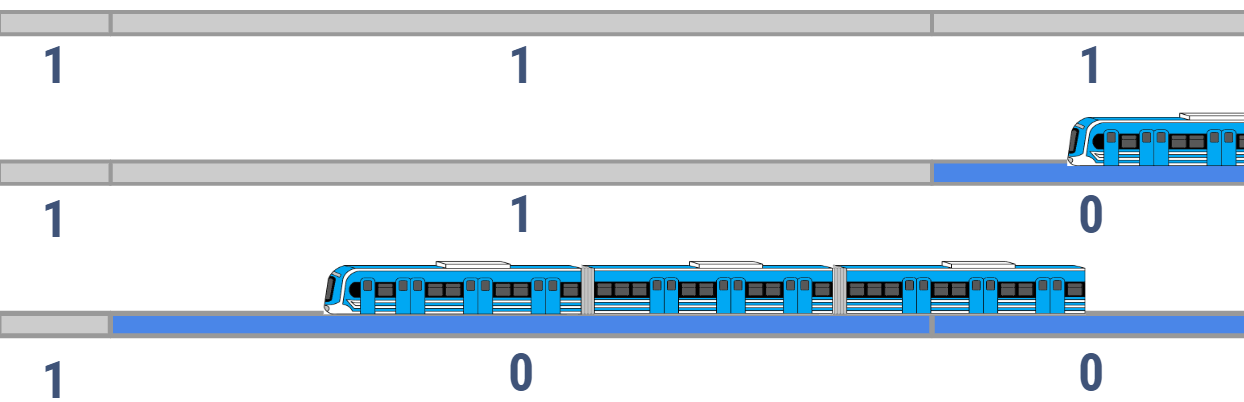
\includegraphics[width=1\textwidth]{Figuras/circuito_via}
        \centering\caption{Circuito de vía libre y ocupado.}
        \label{fig:deteccion_1}
    \end{figure}

En caso de que la alimentación se interrumpa, el cableado sufra alguna falla, vandalismo, inundación, o que efectivamente una formación ocupe la sección, el circuito de vía reportará que la sección se encuentra ocupada. De esta manera, solo es posible recibir un reporte de sección desocupada cuando la sección efectivamente se encuentre desocupada. A este principio se le denomina fail-safe [REF]. Es decir, si por alguna razón algo falla, el sistema adopta la condición más restrictiva, mitigando la posibilidad de una situación peligrosa

Los sistemas contadores de ejes (Figura \ref{fig:deteccion_2}) consisten en sensores pasivos instalados en la cara interna de unos de los rieles y un sistema externo de procesamiento de datos. Estos sistemas no dependen de la aplicación de tensiones en la vía. Además, no solo permiten detectar la presencia de una formación, sino que también pueden usarse para medir la integridad de la formación, sabiendo el largo esperado de la misma. 

    \begin{figure}[!h]
        \centering
        \includegraphics[width=1\textwidth]{example-image}
        \centering\caption{Contadores de ejes.}
        \label{fig:deteccion_2}
    \end{figure}

Al igual que los circuitos de vía, los sistemas contadores de eje siguen el principio de fail-safe, adoptando la condición mas restrictiva en caso de falla. Ambos sistemas pueden utilizarse en simultáneo, de ser requerido.
\subsubsection{Estaciones ferroviarias}

Las estaciones ferroviarias son las zonas donde las formaciones pueden detenerse para que los pasajeros puedan descender y nuevos pasajeros puedan abordar. En función del tamaño de las formaciones y la geografía del lugar, las plataformas desde donde ascienden y descienden los pasajeros pueden estar elevadas con respecto al suelo o a ras del mismo. El largo de las plataformas también depende de la cantidad de coches de las formaciones.

Como puede verse en la Figura \ref{fig:estacion_1}, las estaciones ferroviarias incluyen no solo a las plataformas, sino que también pueden centralizar el control de varias operaciones logísticas como la asignación de rutas. No obstante, en este trabajo nos referiremos a las estaciones como plataformas indistintamente.

    \begin{figure}[!h]
        \centering
        \includegraphics[width=1\textwidth]{example-image}
        \centering\caption{XXXXX.}
        \label{fig:estacion_1}
    \end{figure}

Las estaciones de mayor complejidad o de mayor convergencia de ramales suelen concentrar el control de la estación donde se encuentran y varias estaciones vecinas. Las estaciones terminales, a menudo, pueden incluso tener control total de varios ramales completos.
\subsubsection{Cruces ferroviarios}

Los cruces ferroviarios son la intersección entre la vía ferroviaria y una ruta vehicular o peatonal. Estos cruces pueden ser bajo nivel (túnel por debajo de la vía), sobre nivel (puente vehicular por sobre la vía) o a nivel. Un paso a nivel es una zona muy crítica del sistema ferroviario, ya que, a diferencia de un paso sobre nivel o bajo nivel, conviven simultáneamente la formación y el transito vehicular y peatonal. En la Figura \ref{fig:cruce_1} se ilustra la intersección entre el tendido ferroviario, un cruce vehicular y un cruce peatonal.

    \begin{figure}[!h]
        \centering
        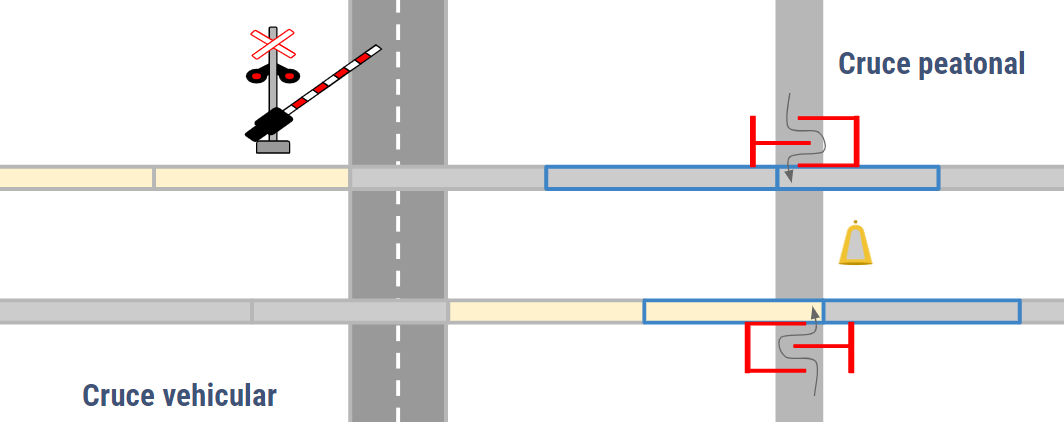
\includegraphics[width=1\textwidth]{Figuras/cruce}
        \centering\caption{XXXXX.}
        \label{fig:cruce_1}
    \end{figure}
    
Los pasos a nivel peatonales incluyen un pequeño laberinto zigzagueante para forzar al peatón a aminorar su marcha y ver a ambos lados antes de cruzar las vías. A menudo suelen estar acompañados de indicaciones lumínicas y sonoras que se accionan tan pronto el tren se encuentre dentro de un rango de varios metros cercano al paso a nivel.

Los pasos a nivel vehiculares añaden barreras ferroviarias para detener el tráfico vehicular cuando un tren se encuentra dentro de un rango de seguridad definido.  El sistema de control de la barrera mantiene el brazo de esta en alto para permitir la circulación vehicular. Si un tren es detectado cerca del paso a nivel, se desenergiza la barrera y comienza a descender el brazo por efecto de la gravedad. Solo cuando la barrera baja, el tren tiene permitido avanzar sobre el cruce, siendo el paso a nivel un sector de altísimo riesgo. Al desocuparse las secciones próximas al paso a nivel, la barrera vuelve a energizarse y se sitúa en estado alto nuevamente, a la espera de otro tren para reiniciar el proceso. 

Se debe destacar que el mismo proceso de descenso de la barrera ocurrirá si esta se desenergiza por una falla electricomecánica y/o pérdida de alimentación. Es decir, el sistema asumirá el estado más seguro ante cualquiera de los mencionados fallos, siguiendo el principio de falla segura.
\subsubsection{Máquina de cambios}

    \lipsum[1]

    \begin{figure}[h]
        \centering
        \includegraphics[width=0.5\textwidth]{example-image}
        \centering\caption{XXXXX.}
        \label{fig:cambios_1}
    \end{figure}

    \lipsum[1]
\subsubsection{Señales ferroviarias}

\lipsum[1]

\lipsum[1]
\includegraphics{example-image}
\lipsum[1]

\subsection{Sistemas de enclavamiento}

A modo de ejemplo, se ilustra en la Figura \ref{fig:enclavamiento_1} un sistema de cambios en una vía simple con bypass. Esto permite que dos formaciones puedan cruzarse en sentidos opuestos sin colisionar.

    \begin{figure}[!h]
        \centering
        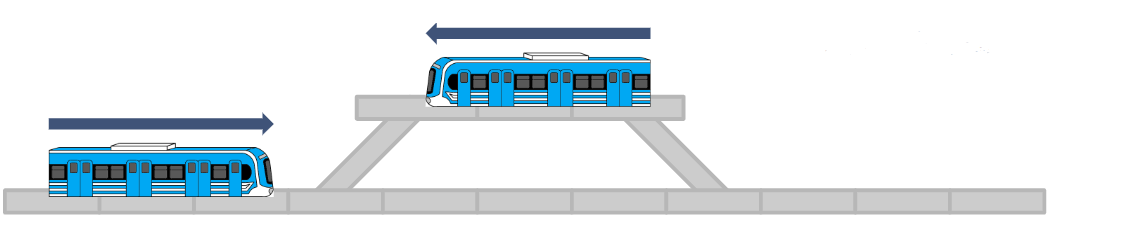
\includegraphics[width=1\textwidth]{Figuras/bypass}
        \centering\caption{XXXXX.}
        \label{fig:enclavamiento_1}
    \end{figure}

Para evitar la colisión, se requiere un control seguro que evite que las formaciones avancen hacia secciones ya ocupadas por otras. También debe evitar que las formaciones avancen sobre los cambios cuando estos aún no han terminado de posicionarse en su lugar, lo que provocaría descarrilamientos. A este control se lo denomina sistema de enclavamiento y, en definitiva, impide que se produzcan configuraciones no seguras y controla los semáforos que habilitan o no los itinerarios de las formaciones. Una falla en un enclavamiento puede poner en peligro cientos de vidas humanas y generar gastos considerables. Por lo tanto, en el diseño del sistema de enclavamiento se deben cumplir estrictos parámetros de fiabilidad, disponibilidad, mantenibilidad y seguridad (RAMS).
    
\subsubsection{Bloqueo de máquina de cambios por ocupación}

\lipsum[1]
\includegraphics{example-image}
\lipsum[1]
\subsubsection{Requerimiento de rutas y bloqueo de cambios en ruta}

\lipsum[1]
\includegraphics{example-image}
\lipsum[1]
\subsubsection{Proteccion por aproximacion}

\lipsum[1]
\includegraphics{example-image}
\lipsum[1]
\subsubsection{Proteccion por solape}

\lipsum[1]
\includegraphics{example-image}
\lipsum[1]
\subsubsection{Doble recubrimiento}

\lipsum[1]
\includegraphics{example-image}
\lipsum[1]
\subsubsection{Liberación secuencial}

\lipsum[1]

    \begin{figure}[!h]
        \centering
        
\includegraphics[width=1\textwidth]{Figuras/secuencial_1}
        \centering\caption{Liberación secuencial.}
        \label{fig:secuencial_1}
    \end{figure}
    
\lipsum[1]

    \begin{figure}[!h]
        \centering
        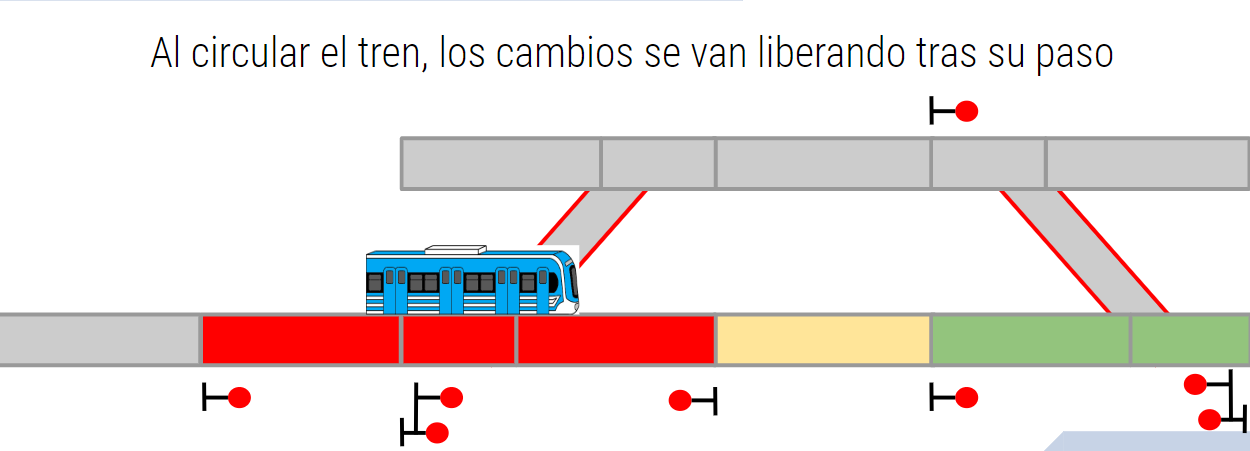
\includegraphics[width=1\textwidth]{Figuras/secuencial_2}
        \centering\caption{Liberación secuencial.}
        \label{fig:secuencial_2}
    \end{figure}
    
\lipsum[1]

    \begin{figure}[!h]
        \centering
        
\includegraphics[width=1\textwidth]{Figuras/secuencial_3}
        \centering\caption{Liberación secuencial.}
        \label{fig:secuencial_3}
    \end{figure}
    
\lipsum[1]

    \begin{figure}[!h]
        \centering
        
\includegraphics[width=1\textwidth]{Figuras/secuencial_4}
        \centering\caption{Liberación secuencial.}
        \label{fig:secuencial_4}
    \end{figure}
    
\lipsum[1]
\subsection{Topologias ferroviarias}

\subsubsection{Simple}

\lipsum[1]
\includegraphics{example-image}
\lipsum[1]
\subsubsection{Bypass}

\lipsum[1]

    \begin{figure}[h]
        \centering
        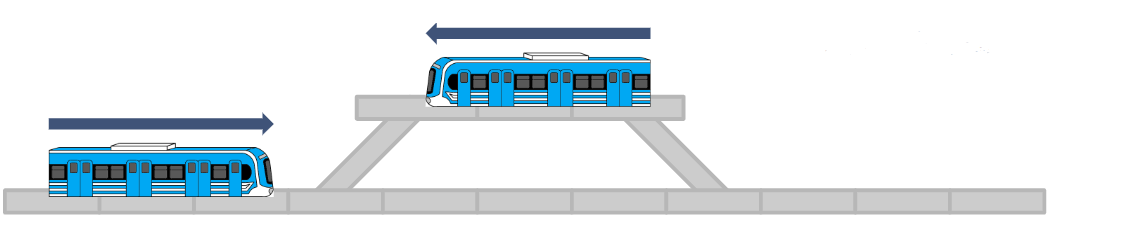
\includegraphics[width=1\textwidth]{Figuras/bypass}
        \centering\caption{Topología bypass.}
        \label{fig:bypass_1}
    \end{figure}
    
\lipsum[1]
\subsubsection{Hub}

\lipsum[1]

    \begin{figure}[h]
        \centering
        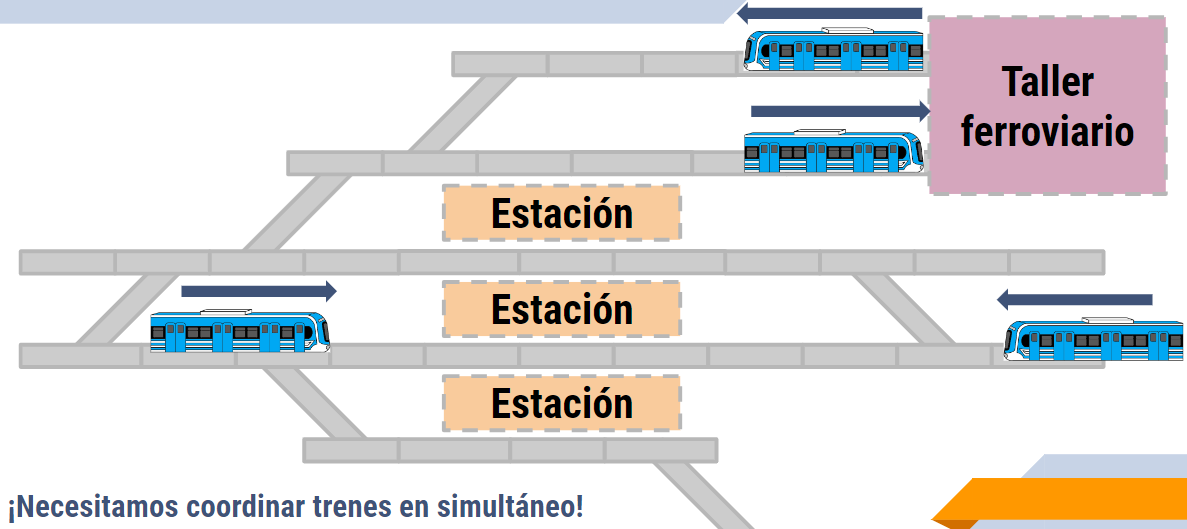
\includegraphics[width=1\textwidth]{Figuras/hub}
        \centering\caption{Topología hub.}
        \label{fig:hub_1}
    \end{figure}
    
\lipsum[1]
\subsubsection{Terminal}

\lipsum[1]

    \begin{figure}[h]
        \centering
        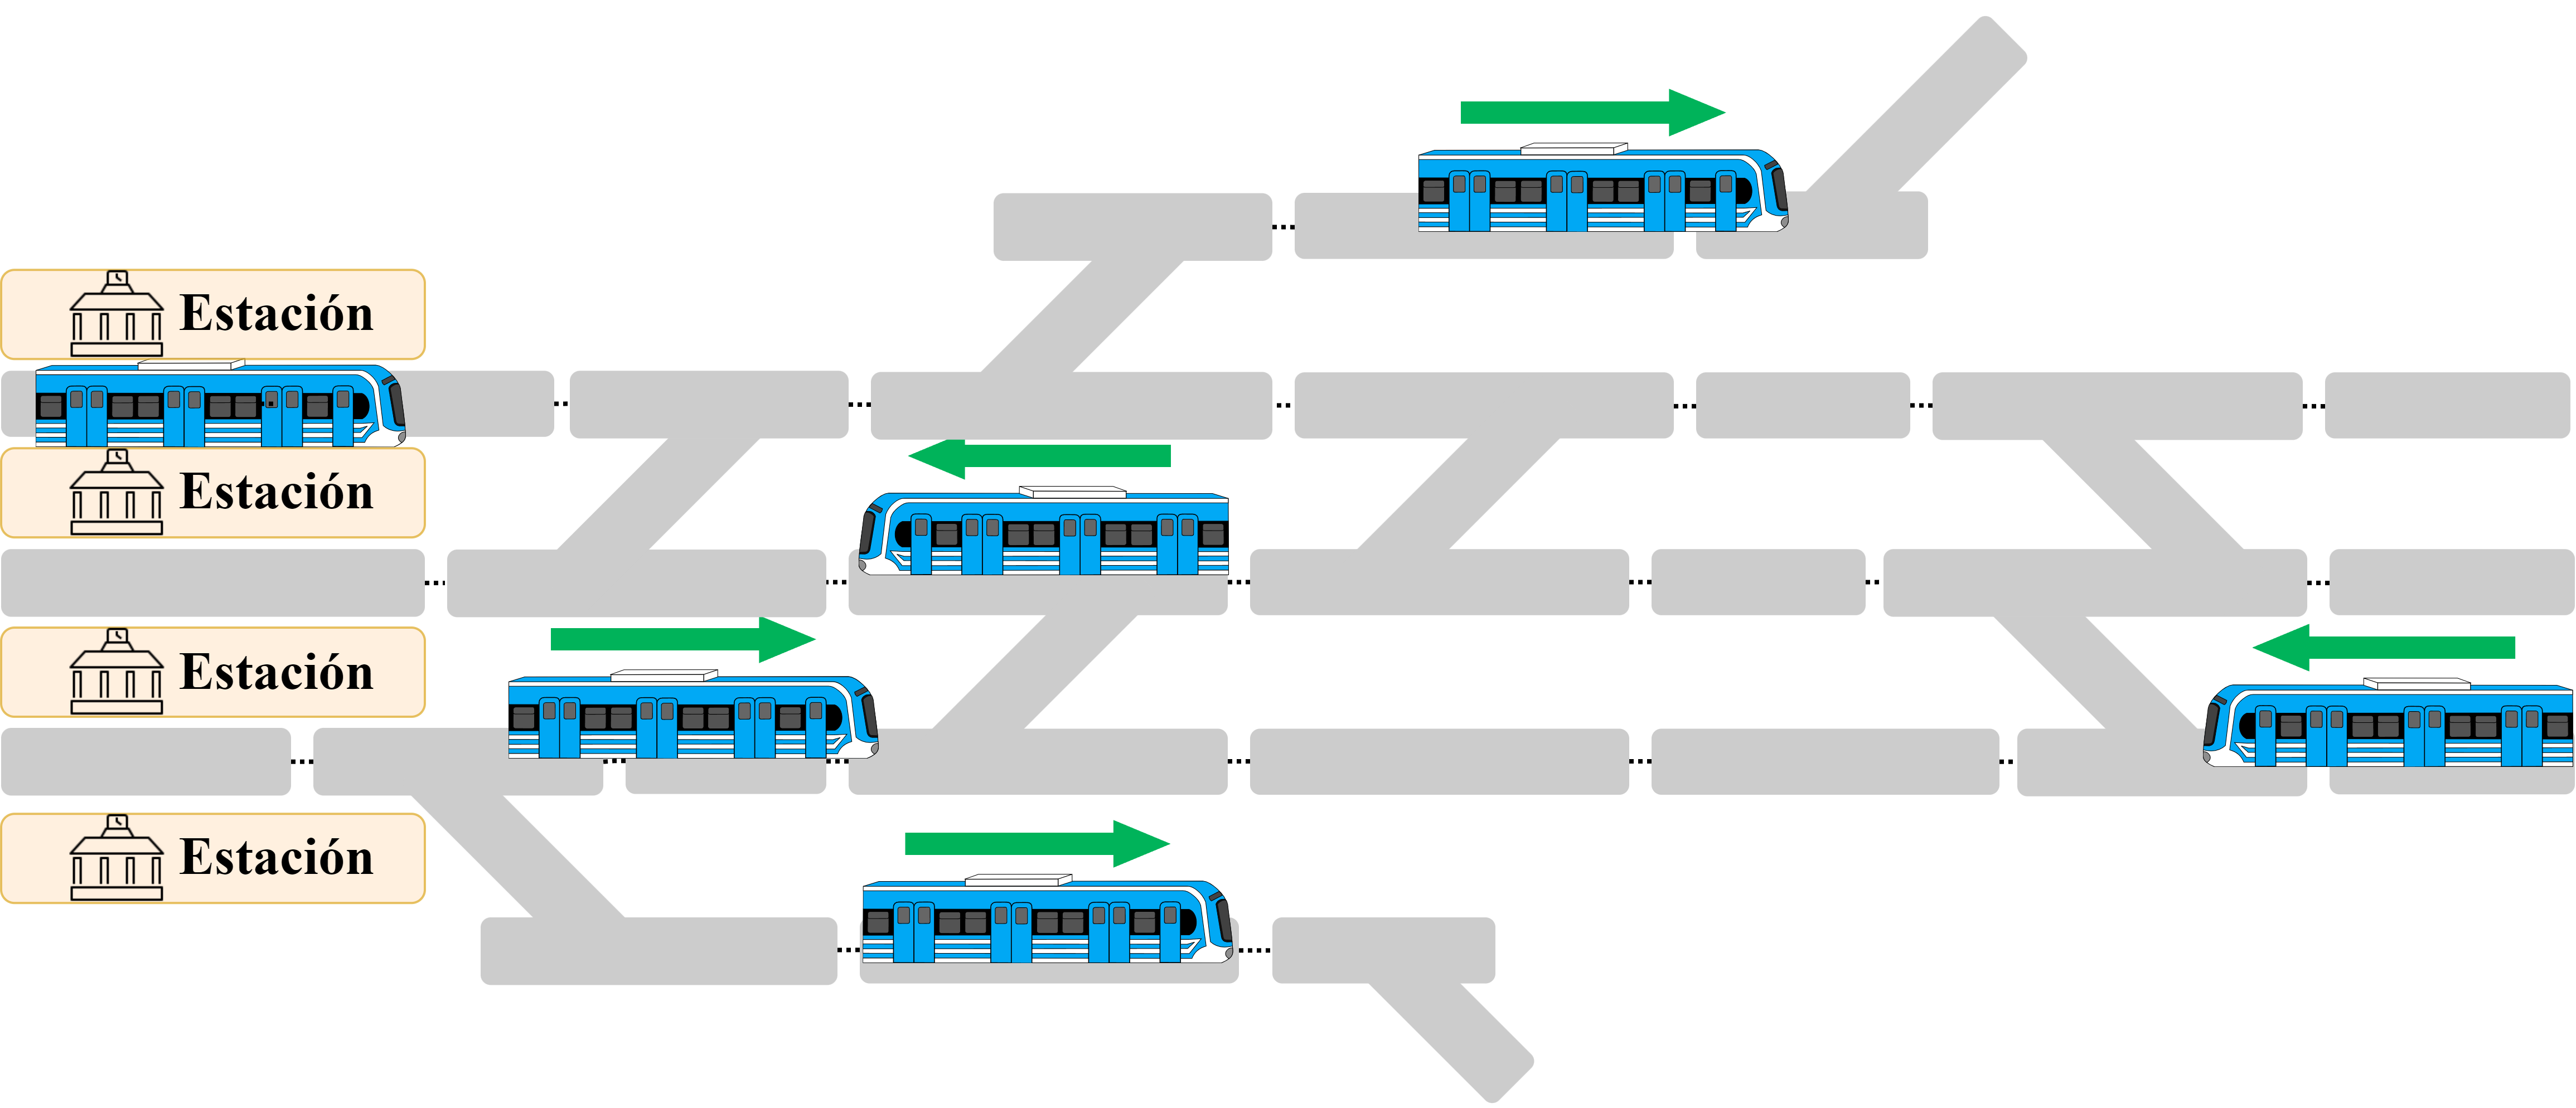
\includegraphics[width=1\textwidth]{Figuras/terminal}
        \centering\caption{Topología terminal.}
        \label{fig:terminal_1}
    \end{figure}
    
\lipsum[1]
\subsubsection{Complejas}

\lipsum[1]
\includegraphics{example-image}
\lipsum[1]
\section{Estado del arte}

\lipsum[1]

\subsection{Empresas del sector ferroviario}

\lipsum[1]
\subsection{Herramientas existentes}

\lipsum[1]
\subsection{Estudios realizados}

\lipsum[1]
\subsection{Enfoque funcional vs enfoque geografico}

\lipsum[1]

\subsection{RailTopoModel}

\lipsum[1]

\subsubsection{Modelo de grafos}

\lipsum[1]
\subsubsection{Topología y niveles}

    La topología del modelo es una parte fundamental del estándar. RailTopoModel incluye el "principio de agregación", por el cual los elementos pueden ser agrupados en entidades mas grandes. En la Figura \ref{fig:RTM_1} se puede visualizar la estructura de capas propuesto por RailTopoModel.

    \begin{figure}[!h]
        \centering
        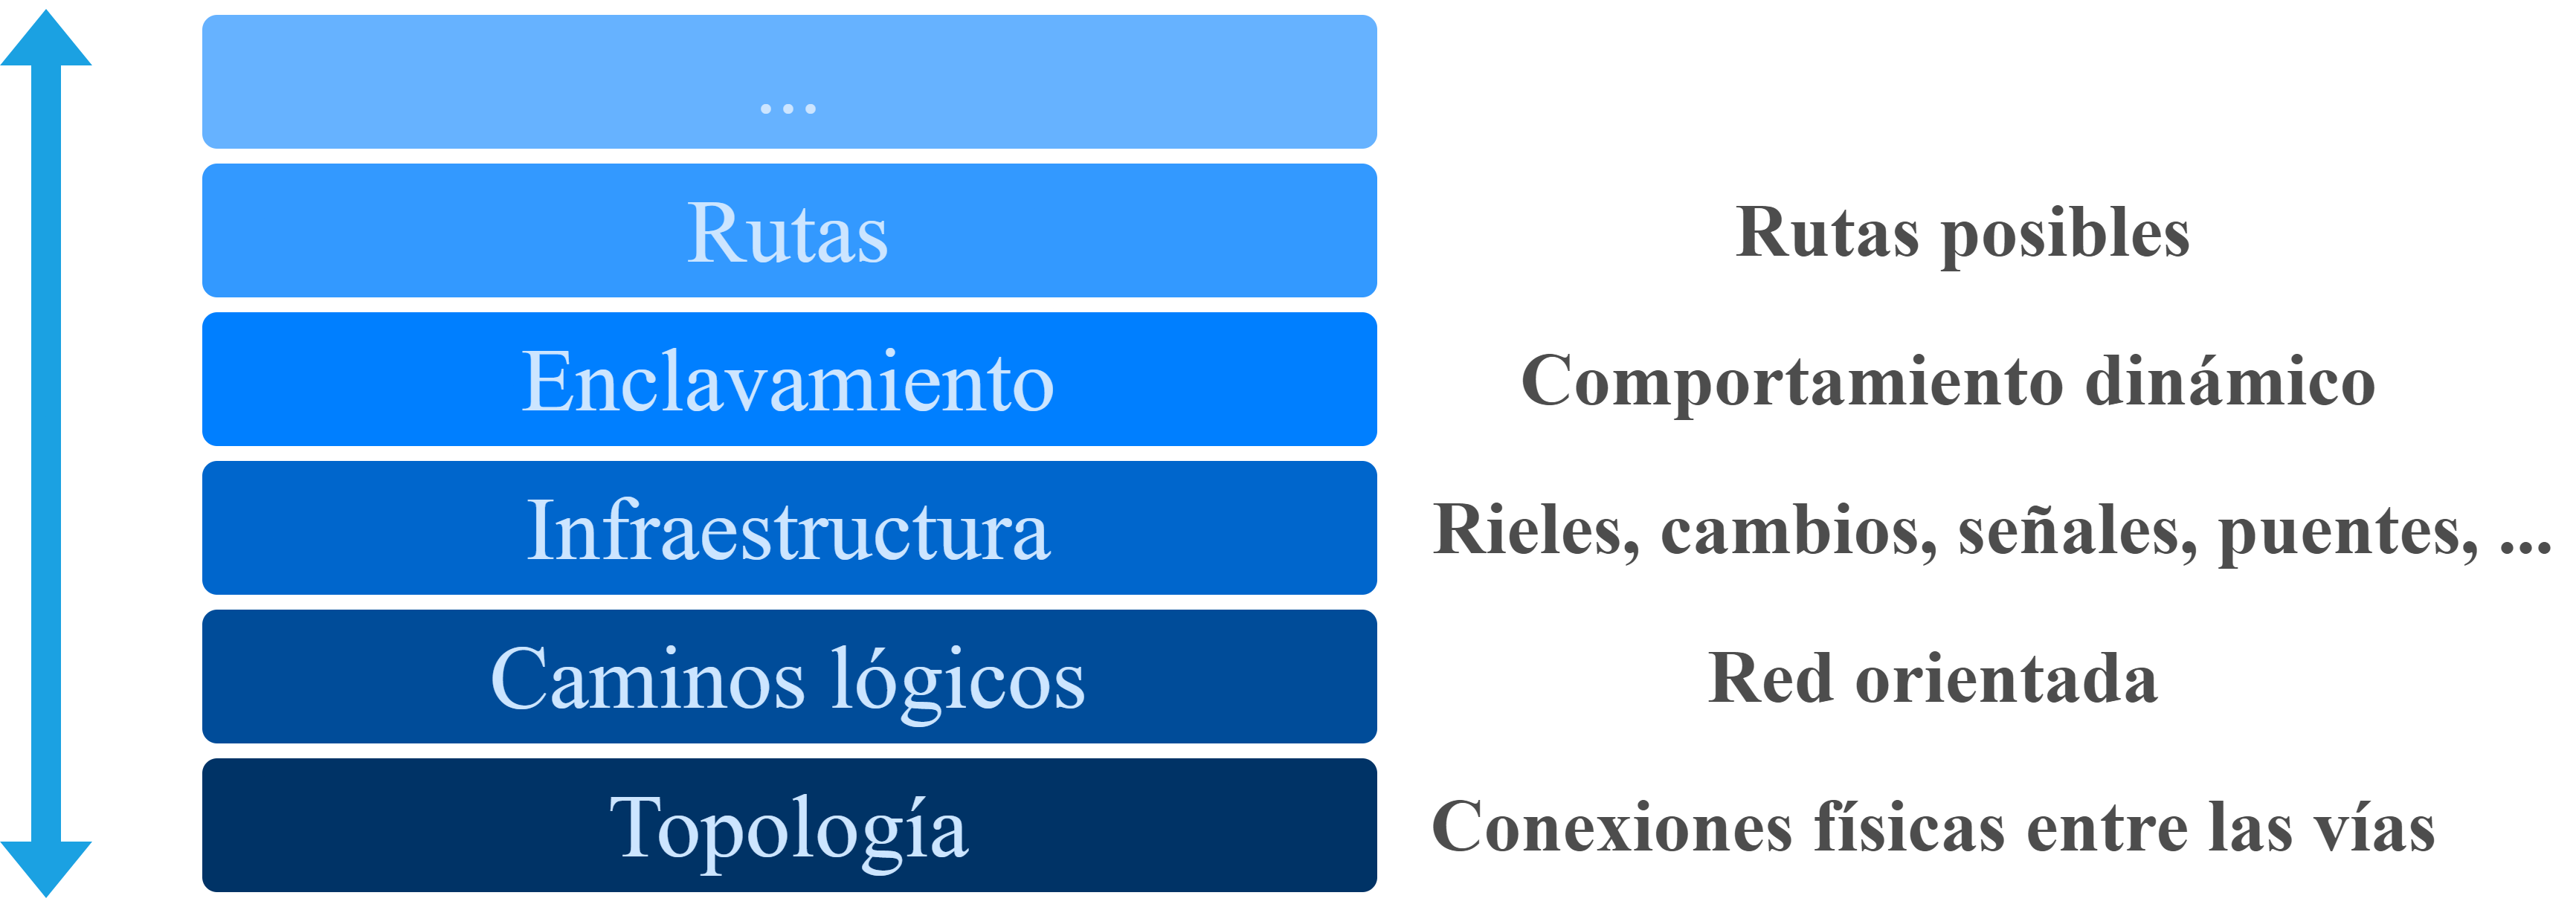
\includegraphics[width=1\textwidth]{Figuras/capas}
        \centering\caption{Estructura de capas de RailTopoModel.}
        \label{fig:RTM_1}
    \end{figure}
    
    La topología de la red está compuesta por los nodos (netElements) y las aristas (netRelations) que los conectan entre sí, lo cual constituye el nivel microscópico de la red. Cada nodo representa un tramo de vías que puede tener ciertos elementos ferroviarios asociados o ninguno. A su vez, los nodos pueden ser agrupados en diversos caminos lógicos, que son el conjunto de nodos cuyas relaciones y navegabilidad les permite constituir un camino físico entre ellos.

    A medida que se agrupan mas y mas cambios de vías junto con las plataformas y máquinas de cambios se constituye un punto de operación. La descripción en base a puntos de operación es a nivel mesoscópico, como se muestra en la Figura \ref{fig:RMT_2}, y es utilizado en logística. Las secciones de vía que no incluyen plataformas en las cuales las formaciones puedan detenerse se denominan secciones de líneas, o simplemente "líneas" dentro del modelo de RailTopoModel. La descripción que incluye tanto los puntos de operación como las secciones de líneas es a nivel macroscópico. Esta simplificación de la red es de gran importancia, ya que es ampliamente utilizada en los mapas ferroviarios de todas las estaciones del mundo: los puntos de operación son las estaciones y las secciones de línea son las vías que las comunican. 
    
    \begin{figure}[!h]
        \centering
        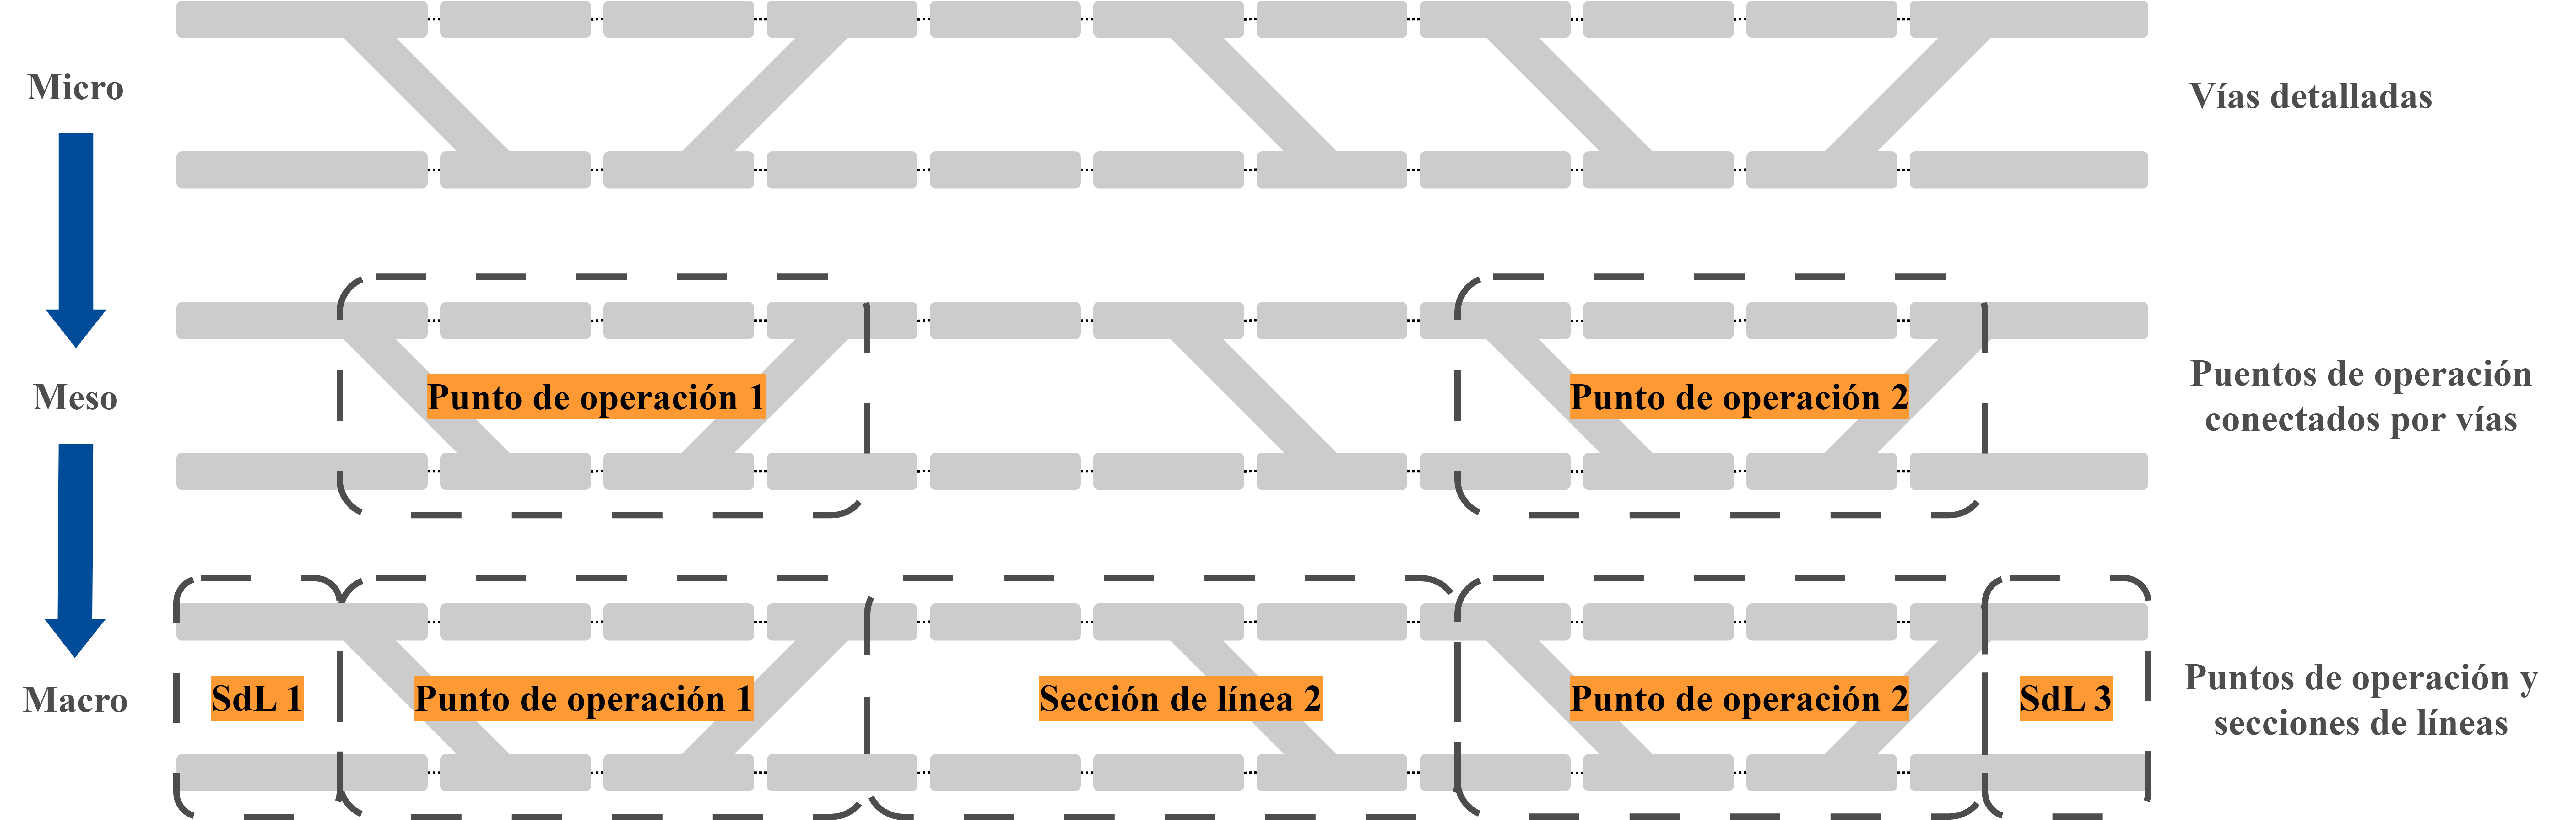
\includegraphics[width=1\textwidth]{Figuras/railtopomodel}
        \centering\caption{Niveles microscópico, mesoscópico y macroscópico.}
        \label{fig:RTM_2}
    \end{figure}
    
    Las instalaciones y sus propiedades constituyen todos los elementos ferroviarios asociados a un nodo. Estos representan elementos físicos del mundo real, pueden ser estáticos o dinámicos. Los elementos estáticos como los puentes, curvas y estaciones no alteran sus propiedades en ningún momento. Los elementos dinámicos como los pasos a nivel, máquinas de cambios o señales tienen algunas propiedades fijas, como la posición física del elemento, pero otras variables, como la posición mecánica de alguna de sus piezas o el estado eléctrico de sus circuitos.

    Un sistema de enclavamiento relaciona todos los módulos previamente mencionados. El sistema de enclavamientos modificará el estado de los elementos dinámicos, basados en el estado actual de los mismos, sometido a las restricciones impuestas por los elementos estáticos, buscando habilitar los caminos lógicos mas cortos y seguros entre un punto A y B.

    Finalmente, en base al estado de los elementos dinámicos decidido por el sistema de enclavamiento, buscando el camino óptimo entre A y B que no comprometa la infraestructura del sistema, es que obtenemos las rutas permitidas. Todas las restricciones impuestas por las capas inferiores (caminos lógicos posibles, limitaciones de la infraestructura o estados previos que sean incompatibles con lo pedido) terminan emergiendo como un conjunto de rutas posibles de ser utilizadas, en detrimento de otras que, en ese instante de tiempo, no podrán ser habilitadas hasta que el estado del sistema se modifique.

    Como se puede apreciar, en este modelo, las rutas son una consecuencia de la infraestructura que se tiene y de los estados anteriores del sistema, producto de las rutas previamente pedidas. Un análisis completo de la topología e infraestructura permitiría obtener todo el conjunto de rutas posibles, para cualquier estado alcanzable por el sistema.
\subsection{RailML}
    \label{sec:railML}
    
    railML [REF] (del inglés, Railway Markup Language) es un estándar abierto de comunicación de datos entre herramientas ferroviarias desarrollado por las principales empresas de la industria ferroviaria a partir del año 2002. Las primeras dos versiones del estándar se diseñaron en base al enfoque funcional, pero en 2017 se lanzó railML 3.0, basado en RailTopoModel y, por lo tanto, adoptando un enfoque puramente geográfico.

\subsubsection{RailML 3.0}

\lipsum[1]
\subsubsection{Uso del estándar railML en la industria ferroviaria}

    El estándar railML es promovido por empresas de gran peso en la industria ferroviaria como Siemens, Thales, Alstom, CAF, ADIF y Toshiba, que concentrán la mayoría de la cuota de mercado global [REF]. Adicionalmente, diversas instituciones y organismos ferroviarios a nivel estatal y nacional hacen uso del estándar railML en sus desarrollos ferroviarios [REF], tales como: Queensland Rail, Transdev Deutschland, Transperth, Saudi Railway Company y Transport for New South Wales, entre otras.

    En sus primeros años de vida railML experimentó varios cambios, pero no fue hasta su versión 3.0 con enfoque geográfico que el uso del estándar creció exponencialmente. Entre el 40 y el 60\% de sus usuarios adoptaron el estándar en los últimos siete años [REF].

    Podemos encontrar las herramientas mas diversas basadas en railML: analizadores de infraestructura [MAPREX], planificador logístico para material rodante [IVU], visualizadores de datos [railViVid], planificadores de infraestructura [VIS ALL 3D] y visualizadores/simuladores de infraestructura enclavamiento [D4R]. Muchas de ellas certificadas e intercompatibles entre sí. Aunque la mayoría son herramientas de código cerrado, el estándar railML es abierto y sigue un principio bottom-top: todas las necesidades de la industria son tenidas en cuenta para ser incorporadas en nuevas versiones del estándar, siguiendo el exitoso modelo del estándar USB, Bluetooth y GSM. 
\section{Impacto economico}

\lipsum[1]
\includegraphics{example-image}
\lipsum[1]